\documentclass{article}

\usepackage[russian]{babel}
\usepackage[T2A]{fontenc}
\usepackage[utf8]{inputenc}
\usepackage{amsthm}
\usepackage{kpfonts}
\usepackage{indentfirst}
\usepackage{graphicx}
\usepackage{wrapfig}
\usepackage{tabularx}
\usepackage{subcaption}
\newcolumntype{C}[1]{>{\hsize=#1\hsize\raggedright\arraybackslash}X}
\newcolumntype{I}[1]{>{\hsize=#1\hsize\centering\arraybackslash}X}
\usepackage[
paperwidth = 148 mm,
paperheight = 210 mm,
left = 1 cm,
right = 1 cm,
top = 1 cm,
bottom = 1 cm,
footskip = 0 cm
]{geometry}
\usepackage[
margin = 10pt,
font = footnotesize,
labelfont = bf,
labelsep = endash,
labelfont = bf,
textfont = it,
margin = 0pt,
aboveskip = 4pt,
belowskip = - 6pt]{caption}
\title{Домашнее задание №3}
\author{А.Г. Рухадзе}
\date{08.11.18}
\begin{document}
	\maketitle
	
    \section{Планета-гигант: Сатурн} 
\setlength\parindent{0.75 cm}
\begin{wrapfigure}[12]{r}[1 cm]{0.5\textwidth}
\centering
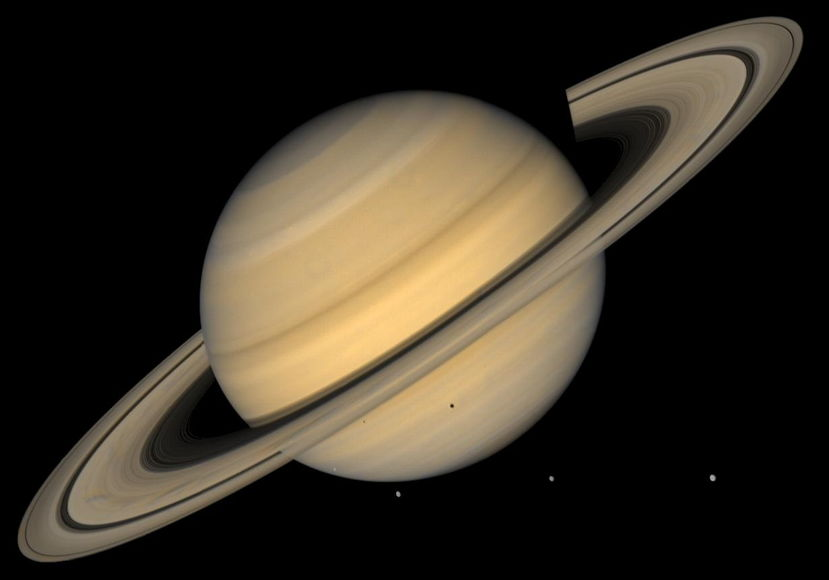
\includegraphics[width = 0.4\textwidth]{img/Saturn}
\caption{Снимок зонда Cassini}
\end{wrapfigure}
Сатурн~--- шестая планета от Солнца и вторая по размерам планета в Солнечной системе после Юпитера. Сатурн, а также Юпитер, Уран и Нептун, классифицируются как газовые гиганты. Сатурн назван в честь римского бога земледелия. \par
В основном Сатурн состоит из водорода, с примесями гелия и следами воды, метана, аммиака и тяжёлых элементов. Внутренняя область представляет собой относительно небольшое ядро из железа, никеля и льда, покрытое тонким слоем металлического водорода и газообразным внешним слоем. Внешняя атмосфера планеты кажется из космоса спокойной и однородной, хотя иногда на ней появляются долговременные образования. \par
\begin{wrapfigure}[12]{l}[- 1 cm]{0.4\textwidth}
\centering
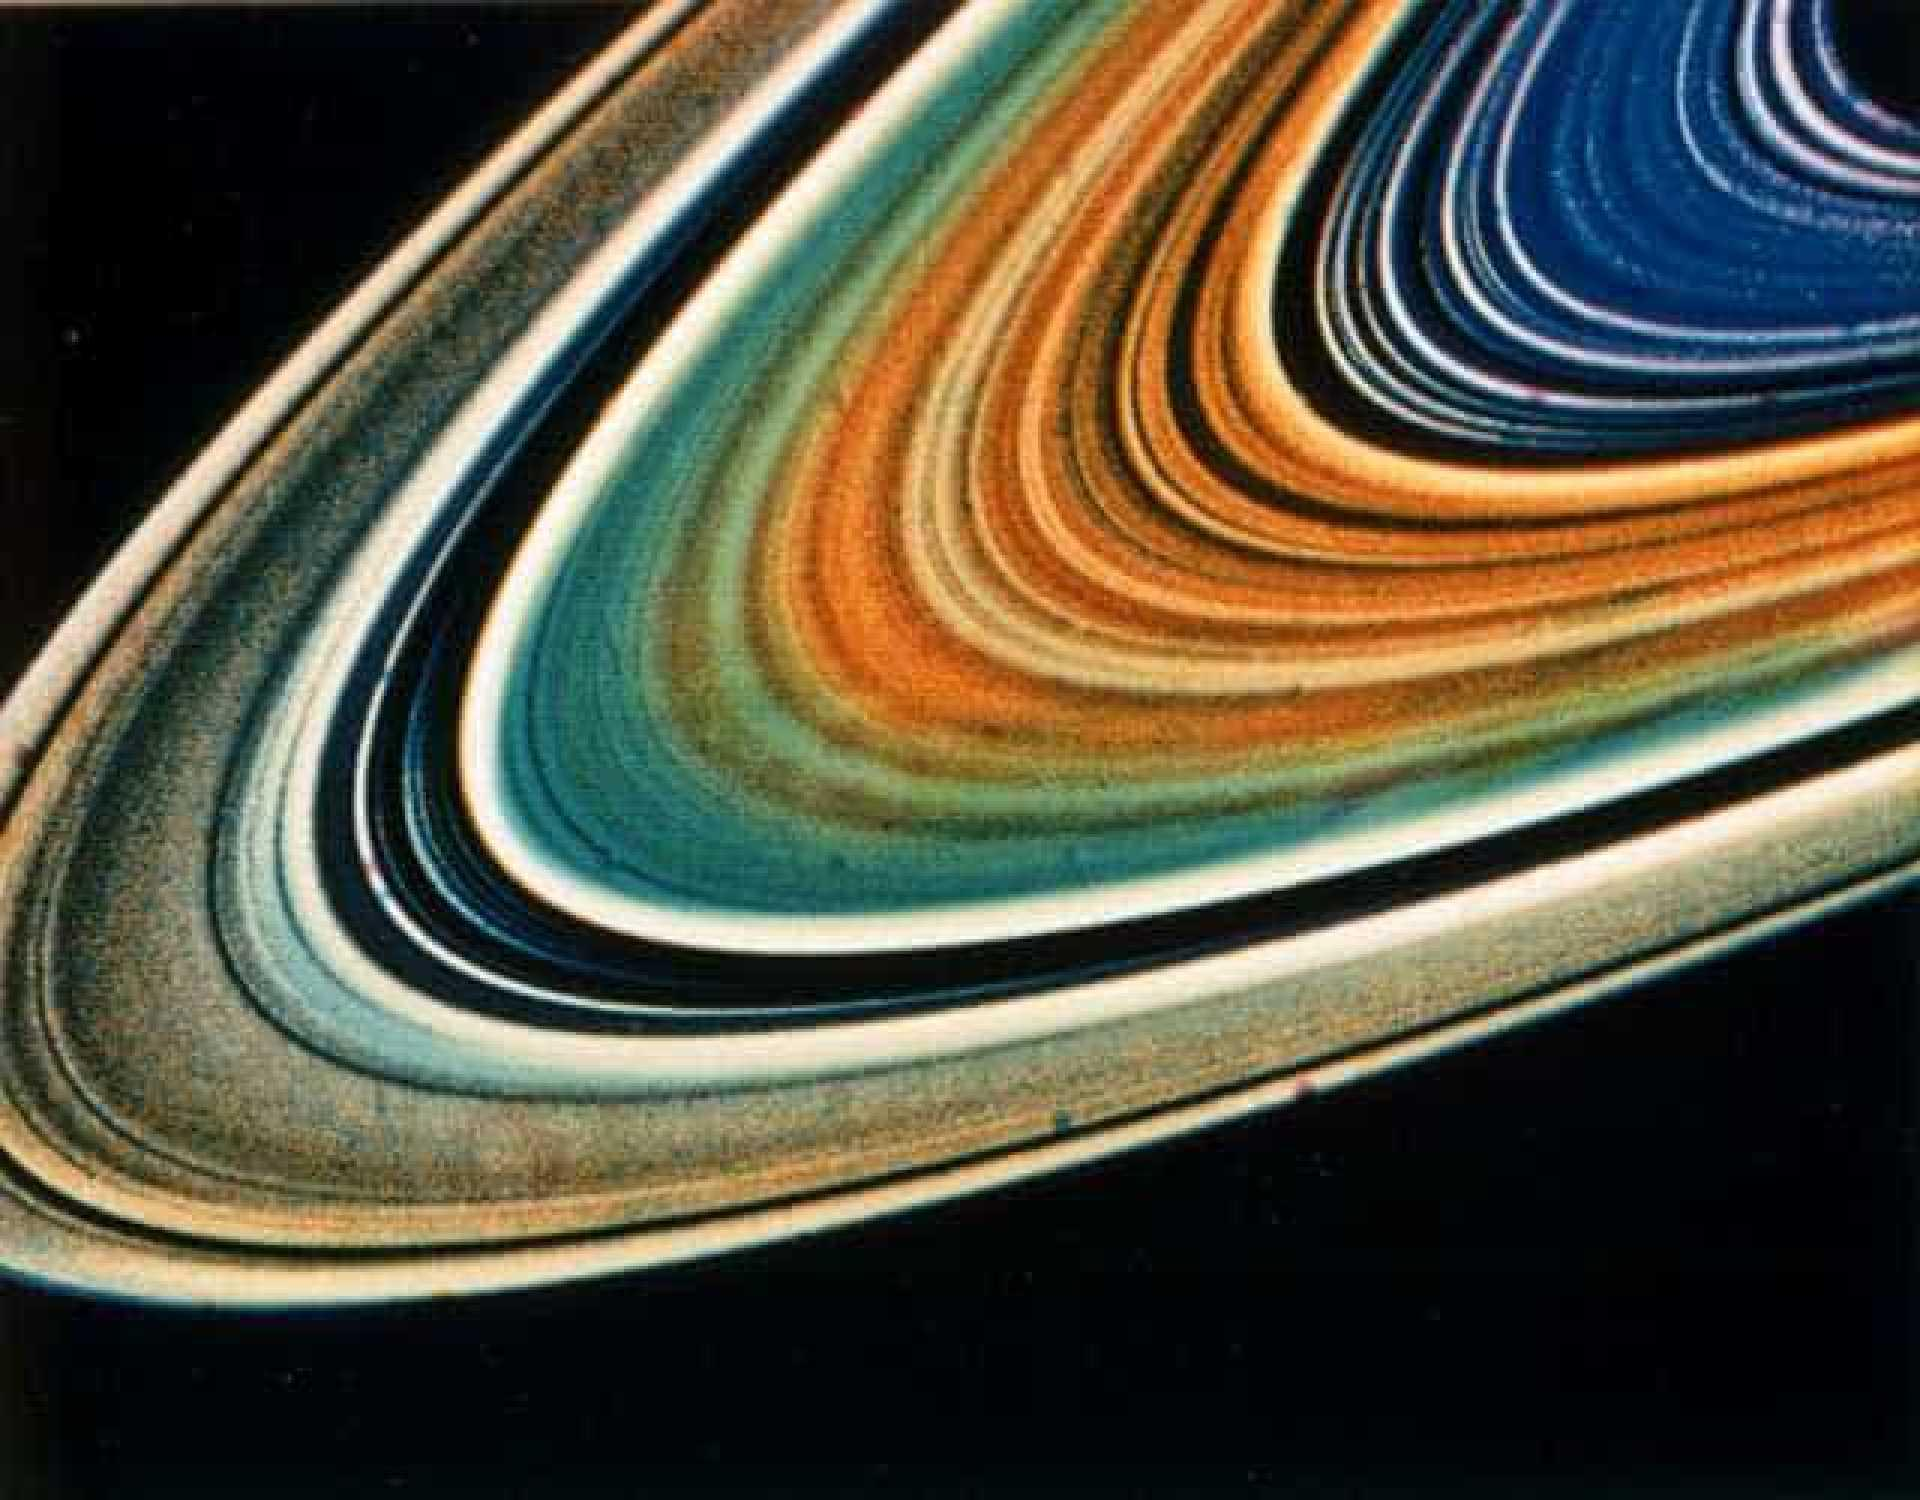
\includegraphics[width = 0.4\textwidth]{img/SaturnRings}
\caption{Кольца Сатурна}
\end{wrapfigure}
    Сатурн известен прежде всего своей главной достопримечательностью~--- кольцами. Издалека нам кажется, что кольцо у Сатурна одно, а на самом деле их четыре: три основных широких и одно очень тонкое. Кольца состоят из обломков льда с примесями различных элементов. Толщина колец по космическим меркам очень мала~--- от нескольких десятков до нескольких сотен метров, хотя их диаметр составляет \\250~тысяч~километров. \par
    Вторая по величине планета в Солнечной системе знаменита своими ветрами, ураганами и бурями. Скорость ветра на Сатурне может достигать 1800~км/ч.
    
    \section{Спутники Сатурна}
    Вокруг планеты обращается 62 известных на данный момент спутника. Титан~— самый крупный из них, а также второй по размерам спутник в Солнечной системе (после спутника Юпитера, Ганимеда), который превосходит по своим размерам Меркурий и обладает единственной среди спутников планет Солнечной системы плотной атмосферой. \par
    Cравнительная характеристика: \par
    \begin{table}[h!]
    \centering
    	\begin{tabularx}{0.95\textwidth}{|C{0.34}|I{0.11}|I{0.11}|I{0.11}|I{0.11}|I{0.11}|I{0.11}|}
    	\hline
     	& Мимас & Тефия & Диона & Рея & Титан & Япет \\
		\hline
		Диаметр, км & 396 & 1062 & 1123 & 1528 & 5151 & 1469 \\
		\hline
		Масса, $10^{20} \text{кг}$ & 0.38 & 7.55 & 10.5 & 24.9 & 1350 & 18.8 \\
		\hline
		Плотность, $\text{г/см}^3$ & 1.15 & 0.984 & 1.48 & 1.24 & 1.88 & 1.09 \\
		\hline
		Расст. до Сатурна, тыс. км & 185.52 & 294.66 & 377.40 & 527.04 & 1221.85 & 3561.3 \\
		\hline
    	\end{tabularx}
    \end{table}
	\section[Казалось бы, при чем тут интегрирование?]{Казалось бы, при чем тут интегрирование?\footnote{За достоверность написанного в данном разделе (да и в других тоже) ответственности не несу.}}
    Перед тем, как ответить на этот вопрос, немножко отвлечемся от астрономии и решим увлекательную задачу: изучим производную кусочнозаданной функции. \par 
    Собственно, вот и сама функция: \par 
    \begin{equation}
    	y = \begin{cases}
    		-(x-4)^2+2, & x \geqslant 4;\\
    		2, & 2 \leqslant x \leqslant 4;\\
    		x, & 1 \leqslant x \leqslant 2;\\
    		x^3, & -1 \leqslant x \leqslant 1;\\
    		-x-2, & x \leqslant -1;\\	
    	\end{cases}
    \end{equation} \par
    Производная данной функции на промежутке $(-\infty,-1) $ будет равняться $-1$: $$ (-x-2)' = -1$$ \par
    Производная данной функции на промежутке $(-1,1) $ будет равняться $3x^2$: $$ \left(x^3\right)' = 3x^2$$ \par
    Производная данной функции на промежутке $(1,2) $ будет равняться $1$: $$ (x)' = 1$$ \par
    Производная данной функции на промежутке $(2,4) $ будет равняться $0$: $$ (2)' = 0$$ \par
    И, наконец, производная данной функции на промежутке $(4,+\infty) $ \\будет равняться $-2(x-4)$: $$ \left(-\left(x-4\right)^2+2\right)' = -2(x-4)$$ \par
    Но чтобы жизнь никому (в первую очередь автору) мёдом не казалась, распишем процесс интегрирования данной функции на отрезке $[-2,6]$. \par 
    \begin{equation}
    	\int\limits_{-2}^{-1} (-x-2)dx =\left.\left(-\frac{1}{2}x^2-2x\right)\right|_{4}^{6} = -\frac{1}{2}; 
    \end{equation}
    \begin{equation}
    	\int\limits_{-1}^{1} \left(x^3\right)dx = \left.\frac{1}{4}x^4\right|_{-1}^{1} = 0;
    \end{equation}
    \begin{equation}
    	\int\limits_{1}^{2} (x)dx = \left.\frac{1}{2}x^2 \right|_{1}^{2} = \frac{3}{2};
    \end{equation}
    \begin{equation}
    	\int\limits_{2}^{4} (2)dx = x\big|_{2}^{4} = 4;
    \end{equation}
    \begin{equation}
    	\int\limits_{4}^{6} \left(-\left(x-4\right)^2+2\right)dx = \left.\left(-\frac{1}{3}x^3+4x^2-14x\right)\right|_{4}^{6} = \frac{4}{3}
    \end{equation} \par 
    Ответим на Ваш вопрос: интегрирование тут вовсе не при чем.
    
    \section{Затмения}
    Затмение~--- астрономическая ситуация, при которой одно небесное тело заслоняет свет от другого небесного тела. \par
    Наиболее известны лунные и солнечные затмения. На~Рис.\ref{pic:types} представлены фото данных видов затмений.
    
    \subsection{Лунные затмения}
    Лунное затмение наступает, когда Луна входит в конус тени, отбрасываемой Землёй. Диаметр пятна тени Земли на расстоянии 363\,000~км (минимальное расстояние Луны от Земли) составляет около 2.5 диаметров Луны, поэтому Луна может быть затенена целиком.
    
    \subsection{Солнечные затмения}
    Солнечное затмение происходит, когда Луна попадает между наблюдателем и Солнцем, и загораживает его. Поскольку Луна перед затмением обращена к нам неосвещённой стороной, то перед затмением всегда бывает новолуние, то есть Луна не видна. Создаётся впечатление, что Солнце закрывается чёрным диском; наблюдающий с Земли видит это явление как солнечное затмение.
    
    
    \begin{figure}[p]
    	\centering
    	\begin{subfigure}[b]{0.45\textwidth}
    		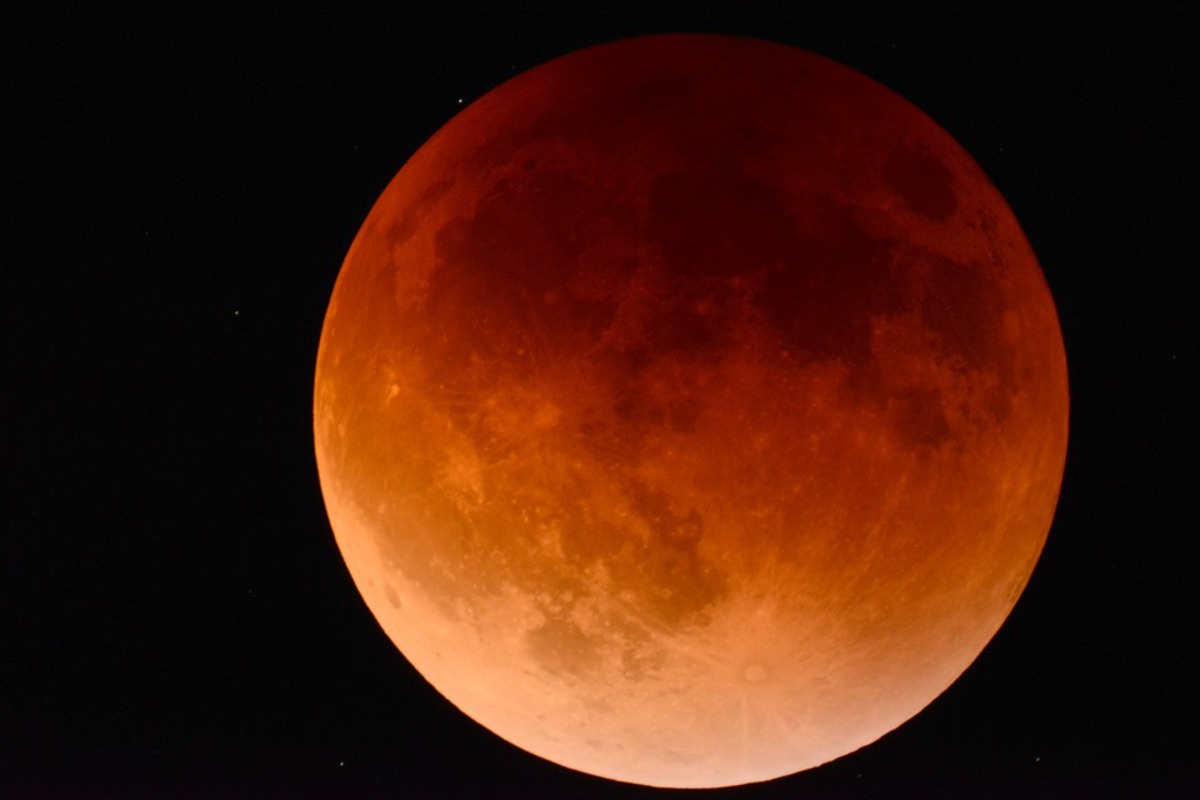
\includegraphics[width = 0.9\textwidth]{img/MoonEclipse}
    		\caption{Лунное затмение}
    	\end{subfigure}
    	\begin{subfigure}[b]{0.45\textwidth}
    		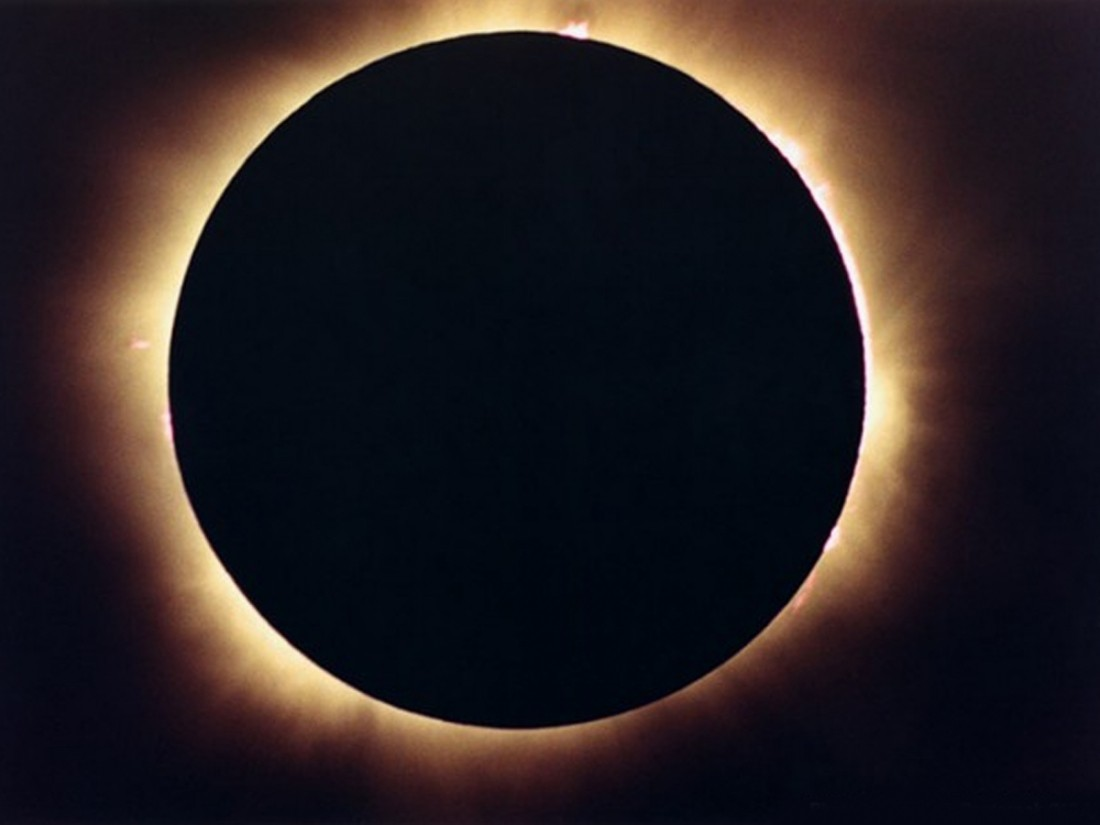
\includegraphics[width = 0.9\textwidth]{img/SunEclipse}
    		\caption{Солнечное затмение}
    	\end{subfigure}
    	\caption{Виды затмений}
    	\label{pic:types}
    \end{figure}
    
    \begin{figure}
    	\centering
    	\begin{subfigure}[b]{0.45\textwidth}
    		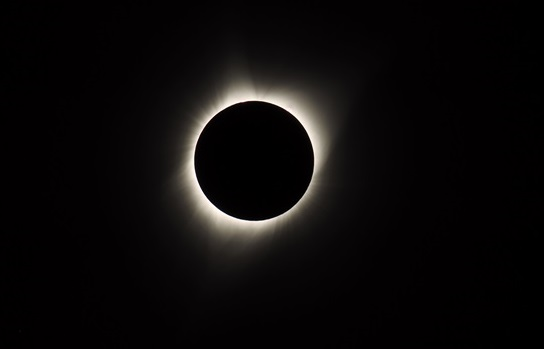
\includegraphics[width = 0.9\textwidth]{img/FullEclipse}
    		\caption{Полное}
    	\end{subfigure}
    	\begin{subfigure}[b]{0.45\textwidth}
    		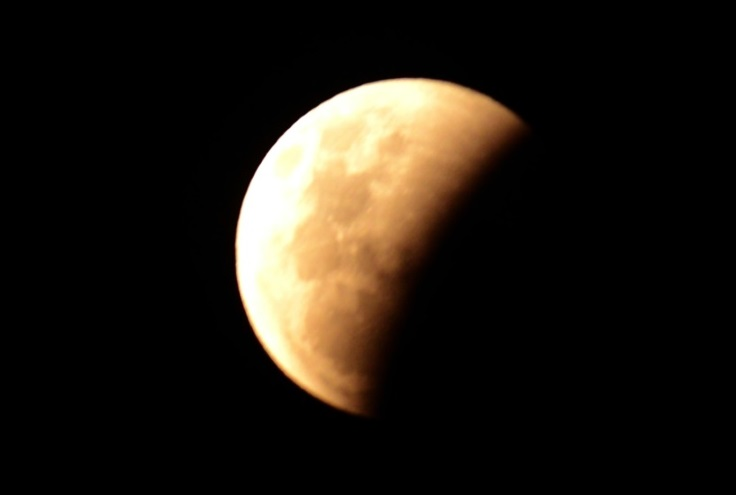
\includegraphics[width = 0.9\textwidth]{img/PartialEclipse}
    		\caption{Частное}
    	\end{subfigure}
    	
    	\begin{subfigure}[b]{0.45\textwidth}
    		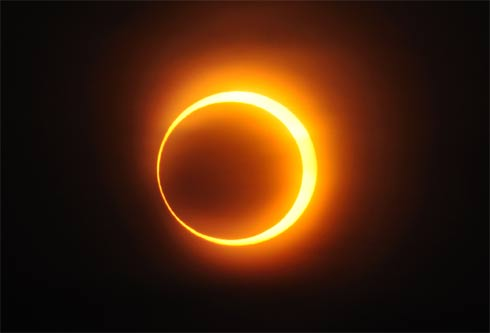
\includegraphics[width = 0.9\textwidth]{img/AnnularEclipse}
    		\caption{Кольцеобразное}
    	\end{subfigure}
    	\begin{subfigure}[b]{0.45\textwidth}
        	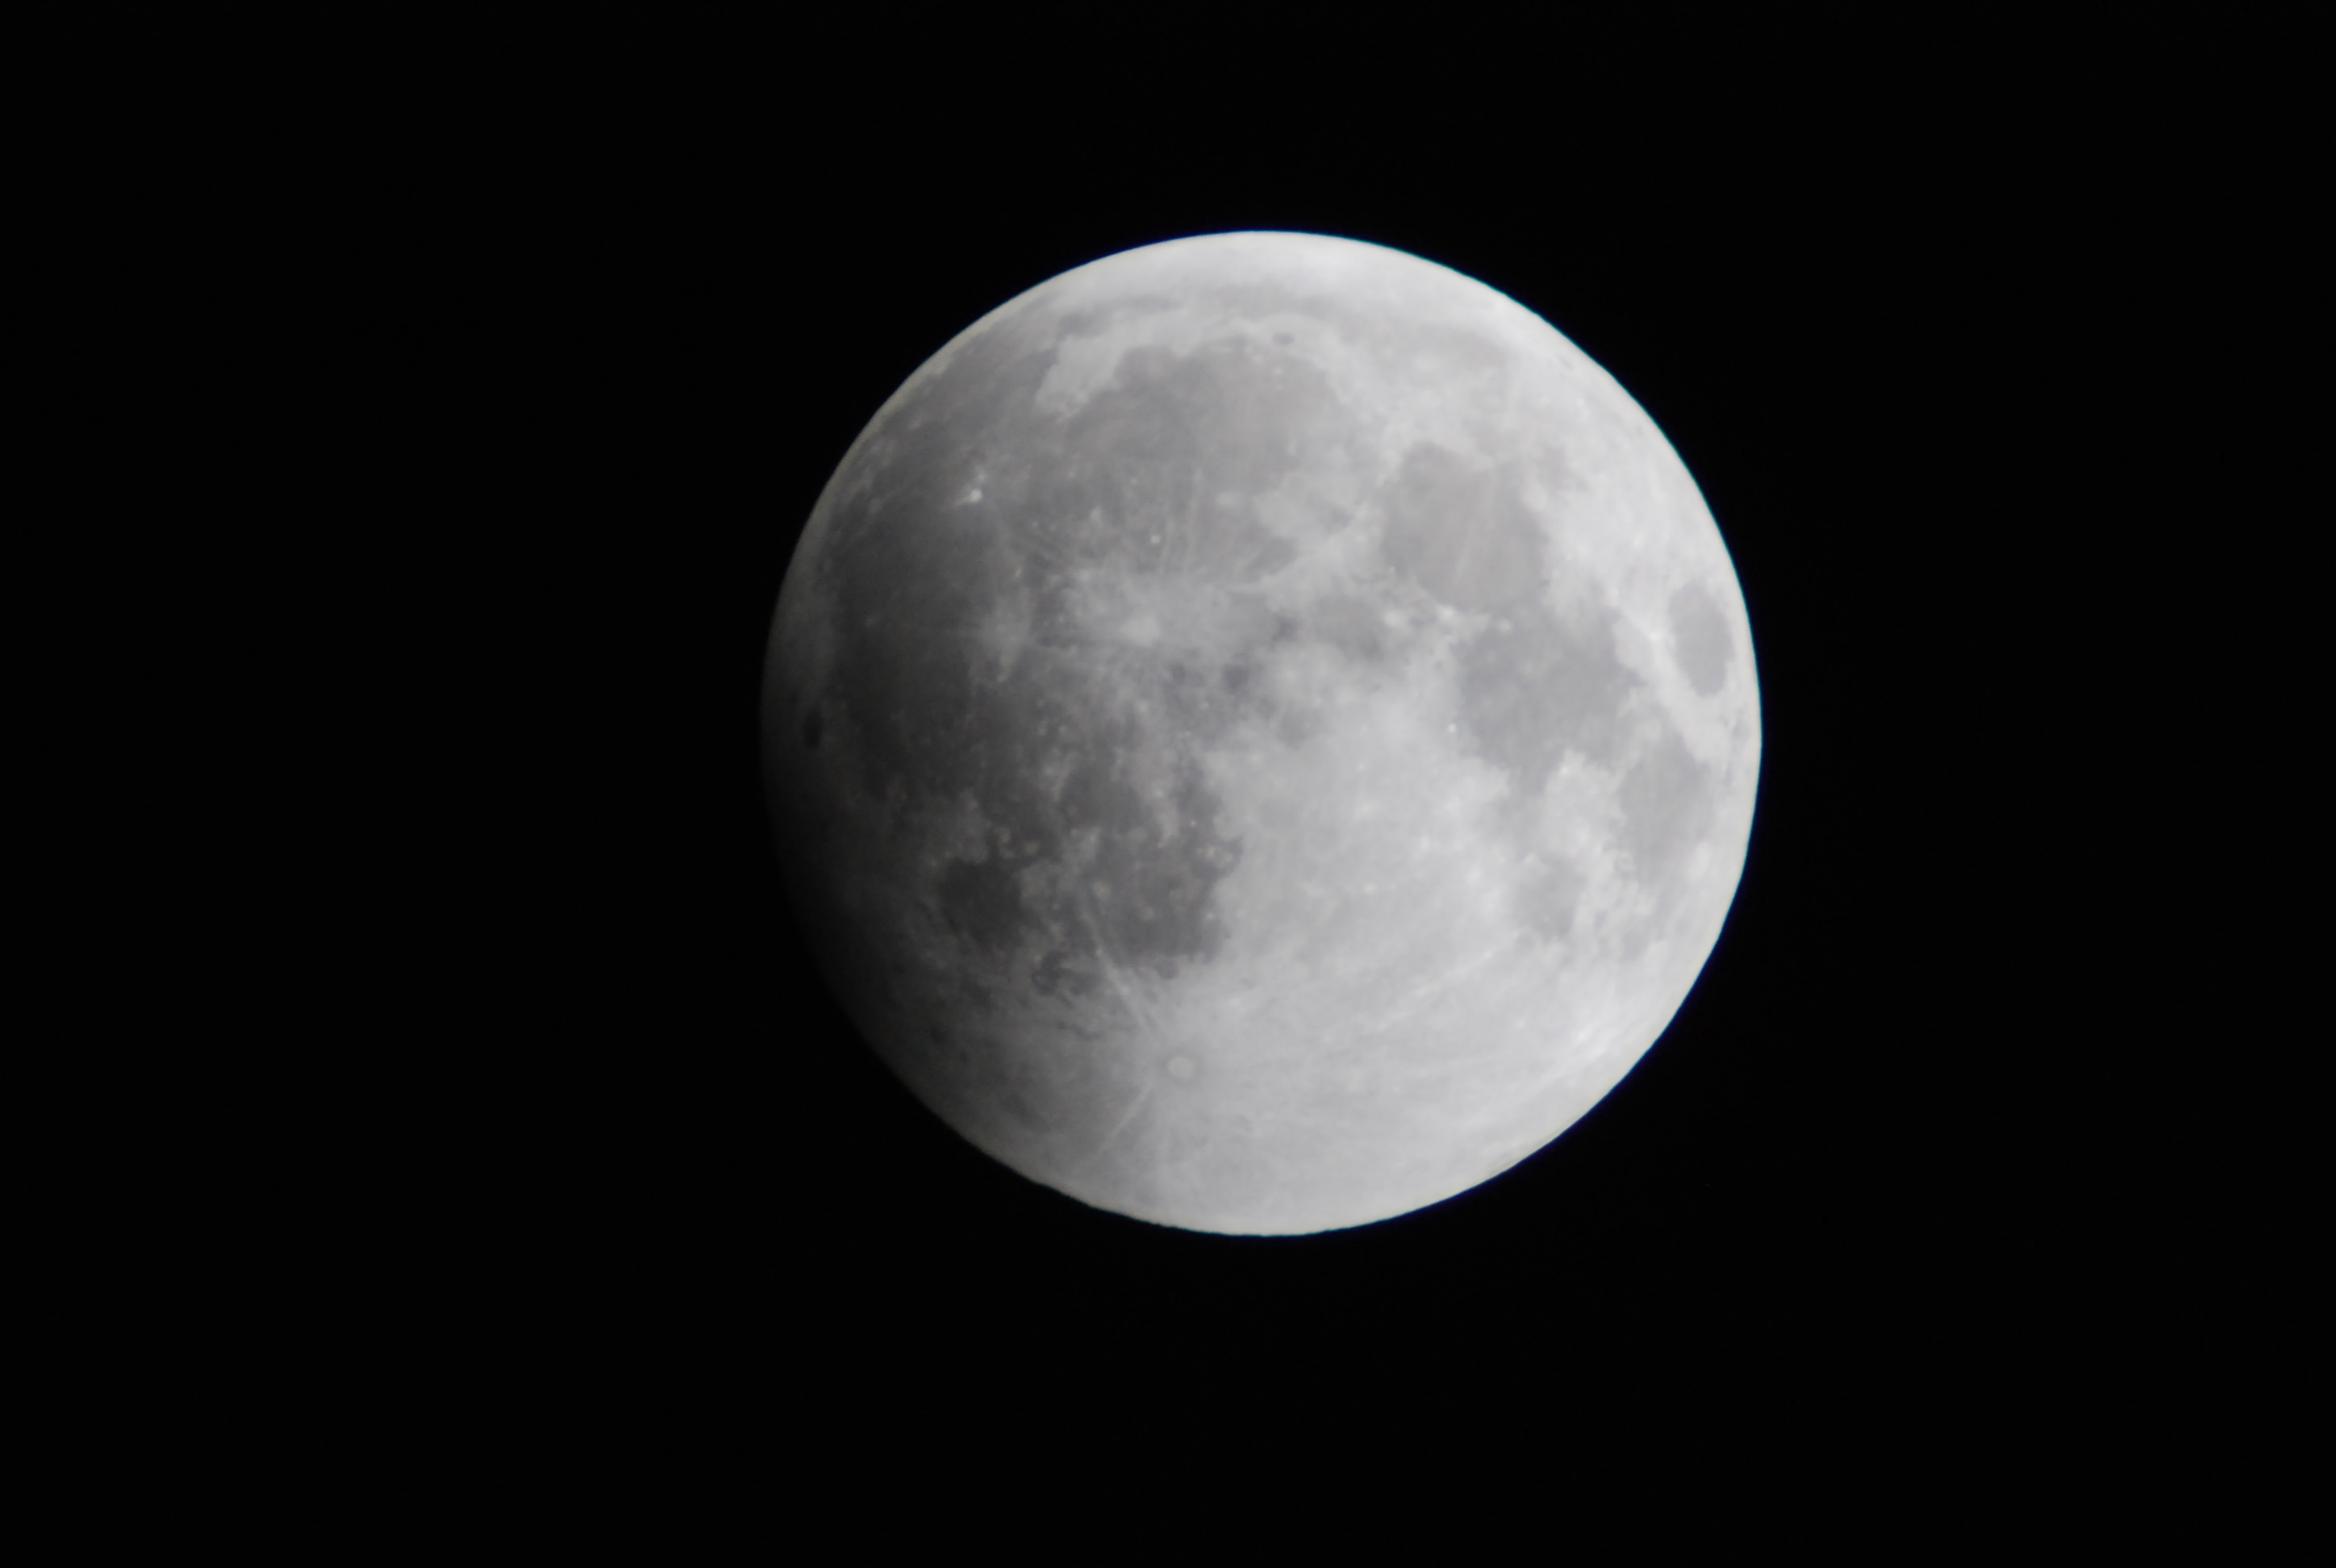
\includegraphics[width = 0.9\textwidth]{img/PenumbralEclipse}
    		\caption{Полутеневое}
    	\end{subfigure}
    	\caption{Виды лунных и солнечных затмений}
    \end{figure}




    
\end{document}